\documentclass[9pt]{beamer}
\usetheme{Ilmenau}
\usepackage{tikz}
\usepackage{graphicx}
\usepackage{xltxtra}
\usepackage{polyglossia}
\defaultfontfeatures{Ligatures=TeX}
\setmainlanguage{greek}
\usepackage{hyperref}
\hypersetup{urlcolor=blue}
\setromanfont{FreeSerif}
\setsansfont{FreeSans}
\setmonofont{FreeMono}
\usepackage[autostyle,english=american]{csquotes}
\MakeOuterQuote{"}
\usepackage{xcolor}
\usepackage{listings}
\lstset{inputpath=/home/thkam/python/telecomsystems}
\usepackage{caption}
\usepackage{subcaption}
\usetikzlibrary{positioning}
\usetikzlibrary{shapes.arrows}
\usepackage{circuitikz}
\usepackage{multicol}

\definecolor{codegreen}{rgb}{0,0.6,0}
\definecolor{codegray}{rgb}{0.5,0.5,0.5}
\definecolor{codepurple}{rgb}{0.58,0,0.82}
\definecolor{backcolour}{rgb}{0.95,0.95,0.92}

\usefonttheme{professionalfonts} % using non standard fonts for beamer
\usefonttheme{serif} % default family is serif
\usepackage{fontspec}
\setmainfont{Liberation Serif}

\lstdefinestyle{mystyle}{
	backgroundcolor=\color{backcolour},   
	commentstyle=\color{codegreen},
	keywordstyle=\color{magenta},
	numberstyle=\tiny\color{codegray},
	stringstyle=\color{codepurple},
	basicstyle=\ttfamily\tiny,        
	breaklines=true,                 
	captionpos=b,                    
	keepspaces=true,                 
	numbers=left,                    
	numbersep=5pt,                  
	showspaces=false,                
	showstringspaces=false,
	showtabs=false,                  
	tabsize=2	
}

\lstset{style=mystyle}


\title{Τηλεπικοινωνιακά Συστήματα}
\subtitle{Διάλεξη 2η}
\author{Θωμάς Καμαλάκης}
\institute{Χαροκόπειο Πανεπιστήμιο Αθηνών}
\date{Οκτώβριος 2020}

\begin{document}
	\begin{frame}
	\titlepage
	\end{frame}
	\begin{frame}
	\frametitle{Περιεχόμενα}
	\tableofcontents
	\end{frame}
	\section{Σήματα}
	\begin{frame}
	\frametitle{Η έννοια του σήματος}
	\begin{itemize}
	\item Στα συστήματα επικοινωνιών μεταδίδουμε αναλογικά και ψηφιακά \emph{σήματα}.
	\item Ενα σήμα $v(t)$ είναι μία μεταβολή ενός μεγέθους $v$ (π.χ. τάση) σε συνάρτηση με το χρόνο $t$ 
	\item Αναλογικό σήμα είναι ένα σήμα που μπορεί να πάρει \emph{οποιαδήποτε τιμή} μέσα σε ένα διάστημα τιμών
	\item Ψηφιακό σήμα είναι ένα σήμα που μπορεί να πάρει \emph{μόνο} κάποιες τιμές.
	\item Παράδειγμα αναλογικού σήματος, $x(t) = A\cos(2\pi f_0t)$.	
	\item Παράδειγμα ψηφιακού σήματος είναι μία bit-σειρά από 0 και 1.	
	\end{itemize}
	\end{frame}
	\begin{frame}
	\frametitle{Ο μετασχηματισμός Fourier}
	\begin{itemize}
		\item Το φάσμα $X(f)$ ενός σήματος αναπαριστά το σήμα στο πεδίο των συχνοτήτων.		
	\end{itemize}
	\begin{equation}
	X(f) = \int_{-\infty}^{+\infty}x(t)\mathrm{e}^{-j2\pi ft}\mathrm{d}t
	\end{equation}	
	\begin{equation}
	x(t) = \int_{-\infty}^{+\infty}X(f)\mathrm{e}^{j2\pi ft}\mathrm{d}f
	\end{equation}	
	\begin{itemize}
	\item Από το σήμα $x(t)$ μπορούμε να υπολογίσουμε το φάσμα $X(f)$.
	\item Από το φάσμα $X(f)$ μπορούμε να υπολογίσουμε το σήμα $x(t)$.
	\end{itemize}	
	\end{frame}

	\begin{frame}
		\frametitle{Παράδειγμα}
		Έστω ένας παλμός $x(t)$ που είναι ίσος με 1 όταν $-T_1/2\le t\le T_1/2$ και ίσος με μηδέν διαφορετικά.
		\begin{multline}
		X(f) = \int_{-\infty}^{+\infty}x(t)\mathrm{e}^{-j2\pi ft}\mathrm{d}t 
		=\int_{-T_1/2}^{+T_1/2}\mathrm{e}^{-j2\pi ft}\mathrm{d}t = \\ 
		=\frac{\mathrm{e}^{j\pi fT_1} - \mathrm{e}^{-j\pi fT_1}}{j2\pi f}
		=\frac{\sin(\pi fT_1)}{\pi f} = T_1 \frac{\sin(\pi fT_1)}{\pi fT_1} 
		=T_1 \mathrm{sinc}(fT_1)
		\end{multline}				
	\end{frame}
	\begin{frame}
	\frametitle{Παράδειγμα}
		Έστω ένας παλμός $x(t)$ που είναι ίσος με 1 όταν $-T_1/2\le t\le T_1/2$ και ίσος με μηδέν διαφορετικά.
		\begin{multline}
		X(f) = \int_{-\infty}^{+\infty}x(t)\mathrm{e}^{-j2\pi ft}\mathrm{d}t 
		=\int_{-T_1/2}^{+T_1/2}\mathrm{e}^{-j2\pi ft}\mathrm{d}t = \\ 
		=\frac{\mathrm{e}^{j\pi fT_1} - \mathrm{e}^{-j\pi fT_1}}{2\pi f}
		=\frac{\sin(\pi fT_1)}{j\pi f} = T_1 \frac{\sin(\pi fT_1)}{\pi fT_1} 
		=T_1 \mathrm{sinc}(fT_1)
		\end{multline}			
		όπου
		\begin{equation}
		\mathrm{sinc}(x) = \left\{
			\begin{array}{ll}
			1 & ,x=0 \\
			\frac{\sin(\pi x)}{\pi x} & ,x\neq 0 
			\end{array}
		\right.
		\end{equation}	
	\end{frame}
	\begin{frame}
		\frametitle{Ένα πρώτο παράδειγμα Python - plotsinc.py}
		\lstinputlisting[language=Python]{lecture2/plotsinc.py}
	\end{frame}

	\section{Ολίγον Python}
	
	\begin{frame}
		\frametitle{Ένα πρώτο παράδειγμα Python - plotsinc.py}
		\begin{figure}
			\begin{subfigure}{0.49\linewidth}
				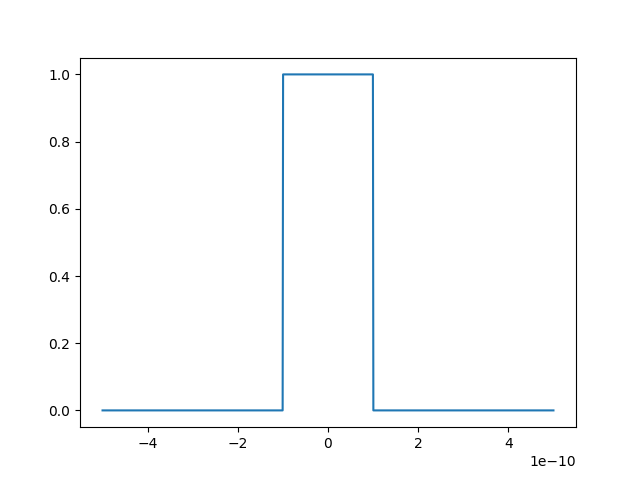
\includegraphics[width=\linewidth]{pulse}
				\caption{figure 1}
			\end{subfigure}	
			\begin{subfigure}{0.49\linewidth}
				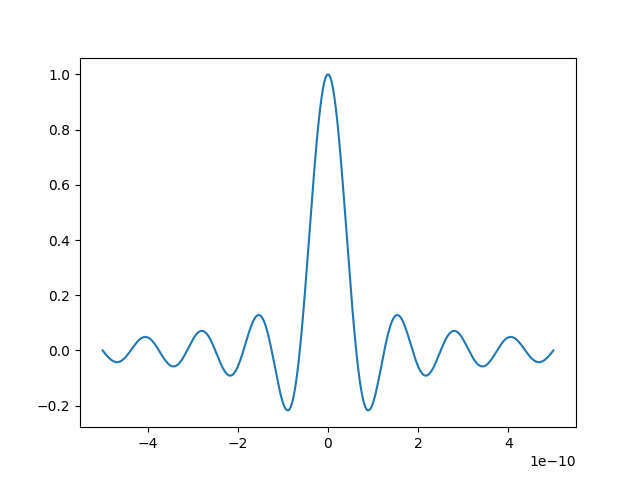
\includegraphics[width=\linewidth]{sinc}
				\caption{figure 2}	
		\end{subfigure}	
		\end{figure}
	\end{frame}
	
	\begin{frame}
		\frametitle{Μερικές επεξηγήσεις}
		\lstinputlisting[language=Python, firstline=1, lastline=2 ]{lecture2/plotsinc.py}
		\begin{itemize}
			\item Στην αρχή κάνουμε import τις βιβλιοθήκες numpy και matplotlib. 
			\item Χρειαζόμαστε την numpy για να χειριστούμε τα σήματα. 
			\item Περιέχει μερικές βασικές συναρτήσεις (π.χ. η sinc κτλ)
			\item Η matplotlib χρησιμοποιείται για τις γραφικές παραστάσεις.
		\end{itemize}	
	\end{frame}	

	\begin{frame}
	\frametitle{Μερικές επεξηγήσεις}
	\lstinputlisting[language=Python, firstline=4, lastline=13 ]{lecture2/plotsinc.py}
	\begin{itemize}
		\item Ορίζουμε ορισμένες παραμέτρους:
		\begin{itemize}
			\item Npt είναι ο αριθμός των σημείων που έχει ο άξονας του χρόνου.
			\item T είναι η διάρκεια του άξονα.
			\item Τ1 είναι η διάρκεια που ο παλμός είναι ίσος με 1.
			\item t είναι ο άξονας του χρόνου.
			\item Npf είναι ο αριθμός των σημείων στον άξονα των συχνοτήτων.
			\item Fmax είναι η μέγιστη συχνότητα που θα έχουμε στον άξονα.
			\item f είναι ο άξονας των συχνοτήτων.
		\end{itemize}
	\end{itemize}	
	\end{frame}

	\begin{frame}
	\frametitle{Μερικές επεξηγήσεις}
	\lstinputlisting[language=Python, firstline=15, lastline=24 ]{lecture2/plotsinc.py}
	\begin{itemize}
		\item Υπολογίζουμε το σήμα στο πεδίο του χρόνου:
		\item φτιάχνουμε ένα πίνακα με όλο μηδενικά, x = np.zeros(t.size).
		\item t.size είναι το μέγεθος του πίνακα t.
		\item μηδενίζουμε έναν counter i
		\item στην ουσία για κάθε τιμή tm στον άξονα αυτόν κοιτάμε να δούμε:
		\begin{itemize}
			\item αν είναι εντός του -Τ1/2 και Τ1/2 τότε θέτουμε ίσο με 1.
			\item αν όχι δεν κάνουμε τίποτα και παραμένει ίσο με μηδέν.
		\end{itemize}
		\item στο πεδίο των συχνοτήτων εφόσον υπάρχει η sinc τα πράγματα είναι πιο εύκολα...		
	\end{itemize}	
	\end{frame}

	\begin{frame}
		\frametitle{Pythonic κώδικας - plotsincen.py}
		\lstinputlisting[language=Python, firstline=16, lastline=20]{lecture2/plotsincen.py}
			\begin{itemize}
			\item Αντί να ορίζουμε έναν counter αφήνουμε την Python να το κάνει για εμάς:
			\item η enumerate επιστρέφει όλα τα στοιχεία τους πίνακες και τους δείκτες τους					
		\end{itemize}		
	\end{frame}

	\begin{frame}
	\frametitle{Python enumerate - enum.py}
	\lstinputlisting[language=Python]{lecture2/enum.py}
	\begin{figure}
	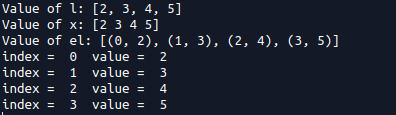
\includegraphics[width=0.7\linewidth]{enumout}
	\end{figure}
	\end{frame}

	\section{Συστήματα}
	\begin{frame}
		\frametitle{Συστήματα}
		\begin{figure}
			\centering
			\begin{tikzpicture}[block/.style={draw, rectangle, minimum height=1cm}]
			\node (box) [block] {Σύστημα}
			node (in1)     [left=-.5cm and 1.0cm of box]     {$x(t)$}
			node (out1)    [right=-.5cm and 1.0cm of box]    {$y(t)$}
			foreach \X in {1}
			{(in\X) edge[->] (box.west |- in\X)
				(box.east |- out\X) edge[->] (out\X)};
			\end{tikzpicture}
		\end{figure}
		\begin{itemize}
			\item Οτιδήποτε επεξεργάζεται ένα σήμα το ονομάζουμε \emph{σύστημα}.
			\item Στην πιο απλή περίπτωση ένα σύστημα έχει μία είσοδο την $x(t)$ και μία έξοδο την $y(t)$.
			\item Η πρώτη υπόθεση που θα κάνουμε είναι ότι το σύστημα είναι \emph{γραμμικό}.
			\begin{itemize}
				\item δηλαδή αν στην είσοδο $x_1(t)$ η έξοδος είναι $y_1(t)$ και στην είσοδο του $x_2(t)$ η έξοδος είναι $y_2(t)$,
				\item τότε η έξοδος που αντιστοιχεί στην είσοδο $c_1x_1(t)+c_2x_2(t)$ όπου $c_1$ και $c_2$ είναι σταθερές, είναι η $c_1y_1(t)+c_2y_2(t)$.
				\item δηλαδή οι συντελεστές $c_1$ και $c_2$ μεταφέρονται από την είσοδο στην έξοδο.
				\item το $c_1x_1(t)+c_2x_2(t)$ ονομάζεται γραμμικός συνδυασμός των $x_1(t)$ και $x_2(t)$.
			\end{itemize}
		\end{itemize}
	\end{frame}

	\begin{frame}
		\frametitle{Συστήματα}
		\begin{figure}
			\centering
			\begin{tikzpicture}[block/.style={draw, rectangle, minimum height=1cm}]
			\node (box) [block] {Σύστημα}
			node (in1)     [left=-.5cm and 1.0cm of box]     {$x(t)$}
			node (out1)    [right=-.5cm and 1.0cm of box]    {$y(t)$}
			foreach \X in {1}
			{(in\X) edge[->] (box.west |- in\X)
				(box.east |- out\X) edge[->] (out\X)};
			\end{tikzpicture}
		\end{figure}
		\begin{itemize}
			\item Μία άλλη κατηγορία συστήματος είναι τα \emph{χρονικά αναλλοίωτα} συστήματα.
			\item στην πράξη ένα χρονικά αναλλοίωτο σύστημα είναι ένα σύστημα στο οποίο η απόκριση δεν εξαρτάται από την χρονική στιγμή που "εισάγουμε" το σήμα εισόδου.
			\item έτσι αν η έξοδος στο $x(t)$ είναι $y(t)$, η έξοδος στο $x(t-t_0)$ είναι $y(t-t_0)$.
		\end{itemize}
	\end{frame}

	\begin{frame}
		\frametitle{Συστήματα στην πράξη}
		\begin{figure}
		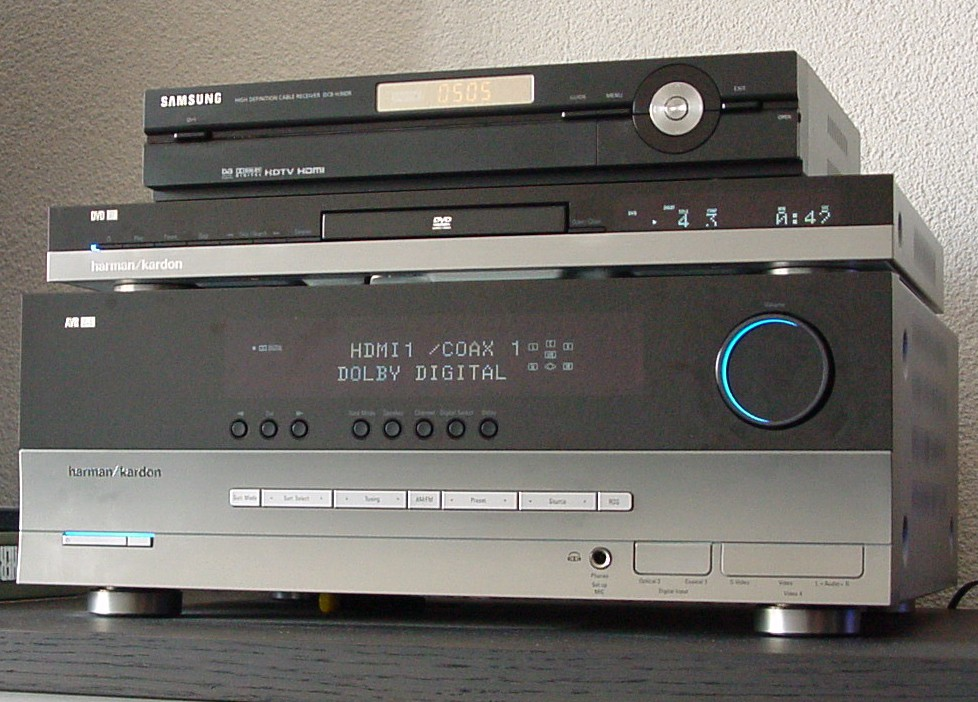
\includegraphics[width=0.35\linewidth]{hifi}
		\end{figure}

		\begin{itemize}
			\item Στην πράξη όλα τα συστήματα \emph{δεν} είναι γραμμικά και \emph{δεν} είναι χρονικά αναλλοίωτα.
			\item Για παράδειγμα, ας θεωρήσουμε τον ενισχυτή του στερεοφωνικού σας.
			\item Αν τερματίσετε την ένταση ακούτε παραμόρφωση. Επομένως η απόκριση στο $cx(t)$ δεν είναι πάντα το $cy(t)$.
			\item Ο ενισχυτής σας δεν είναι γραμμικός!
			\item Επίσης ο ενισχυτής σας μπορεί να "ζεσταθεί" και η απόκριση του να μην είναι η ίδια με αυτή όταν τον ανάψατε.
			\item Επομένως ο ενισχυτής σας δεν είναι χρονικά αναλλοίωτος!
		\end{itemize}
	\end{frame}

	\begin{frame}
	\frametitle{Πως περιγράφονται τα συστήματα;}
	\begin{itemize}		
		\item Ο πρώτος τρόπος είναι στο πεδίο του χρόνου.
		\item Ένα γραμμικό, χρονικά αναλλοίωτο σύστημα χαρακτηρίζεται από αυτό που λέμε "κρουστική απόκριση" $h(t)$.		
		\item Η κρουστική απόκριση καθορίζεται από την φύση του συστήματος.
		\item Αν την ξέρουμε μπορούμε να υπολογίσουμε (επί της αρχής) την έξοδο $y(t)$ σε κάθε είσοδο $x(t)$.
		\begin{equation}
		y(t)=\int_{-\infty}^{+\infty} h(t-\tau)x(\tau)\mathrm{d}\tau		
		\end{equation} 
	\end{itemize}
	\end{frame}

	\begin{frame}
		\frametitle{Κρουστική απόκριση}
		\begin{itemize}
			\item Ας θεωρήσουμε έναν πολύ στενό παλμό $\delta(t)$ που διαρκεί διάστημα $\Delta t$ και έχει πλάτος $\Delta t^{-1}$.
			\begin{equation}
			\delta(t)= \left\{
			\begin{array}{ll}
			\frac{1}{\Delta t} & ,0\le t \le \Delta t \\
			0 & ,\text{διαφορετικά}\\
			\end{array} 
			\right. 
			\end{equation}
		\item αν το σκεφτείτε, είναι ένας "κεραυνός": κτυπάει ακαριαία και με πολύ μεγάλη ένταση (εάν $\Delta t\rightarrow 0$).
		\item Η έξοδος του συστήματος σε αυτή την είσοδο θα είναι:
		\begin{equation}
		y(t)=\int_{-\infty}^{+\infty} h(t-\tau)\delta(\tau)\mathrm{d}\tau=
		\frac{1}{\Delta t}\int_{0}^{\Delta t}h(t-\tau)\mathrm{d}\tau\cong\frac{1}{\Delta t} \Delta th(t) = h(t)		
		\end{equation} 
		\item Παραπάνω θεωρούμε ότι η $h(t)$ δεν μετβάλλεται σημαντικά όταν το $\Delta t$ είναι πολύ μικρό.
		\item Άρα η κρουστική απόκριση είναι η έξοδος του συστήματος όταν βάζουμε έναν πολύ σύντομο παλμό $\delta(t)$ με πολύ μεγάλο πλάτος.
		\end{itemize}		
	\end{frame}

	\begin{frame}
		\frametitle{delta.py}
		\lstinputlisting[language=Python]{lecture2/delta.py}		
	\end{frame}

	\begin{frame}
	\frametitle{delta.py}
	\centering
	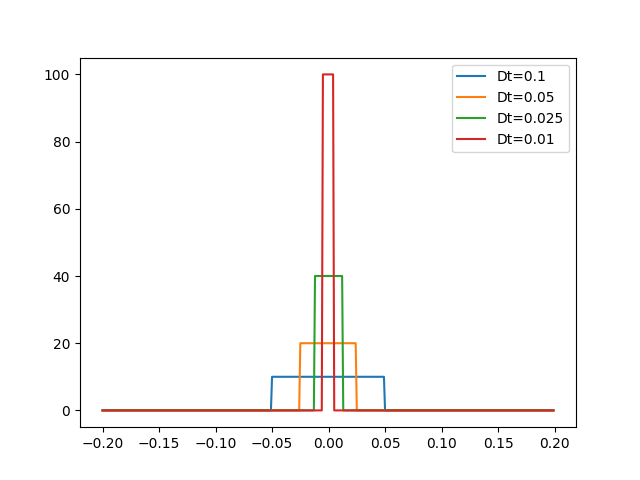
\includegraphics[width=0.7\linewidth]{delta}
	\end{frame}
	
	
	\begin{frame}
		\frametitle{Συστήματα στο πεδίο των συχνοτήτων}
		\begin{itemize}
			\item Η περιγραφή στο πεδίο των συχνοτήτων είναι πιο εύκολη.
			\item Υπολογίζουμε το φάσμα $X(f)$ του $x(t)$.
			\item Υπολογίζουμε το φάσμα $H(f)$ του $h(t)$.
			\item Υπολογίζουμε το φάσμα $Y(f)=H(f)X(f)$.
			\item Υπολογίζουμε το σήμα $y(t)$ από το φάσμα $Y(f)$.			
		\end{itemize}
	\end{frame}
	
	\section{Fast Fourier Transform}
	
	\begin{frame}
		\frametitle{Υπολογίζοντας τα φάσματα χωρίς ολοκληρώματα}
		\begin{itemize}
			\item Πολλές φορές δεν μπορούμε να υπολογίσουμε τα φάσματα
			\item Μπορούμε να δοκιμάσουμε αριθμητική ολοκλήρωση.
			\item Σε αυτό μας βοηθάει ο γρήγορος μετασχηματισμός Fourier - Fast Fourier Transform - FFT.
			\item Στην ουσία προσεγγίζουμε το 
			
			\begin{equation}
			X(f) = \int_{-\infty}^{+\infty}x(t)\mathrm{e}^{-j2\pi ft}\mathrm{d}t
			\end{equation}	
			
			\item με τον διακριτό μετασχηματισμό Fourier,
			
			\begin{equation}
			X_k = \sum_{n=0}^{N-1}x_n\mathrm{e}^{-j\frac{2\pi kn}{N}}
			\end{equation}
					
			\end{itemize}
		\end{frame}
	
	\begin{frame}
		\frametitle{Υπολογίζοντας τα φάσματα χωρίς ολοκληρώματα}
		\begin{itemize}
			\item Θέτουμε $x_n=x(n\Delta t)$ και θεωρούμε το σήμα $x(t)$ σε διακριτές στιγμές $t_n=n\Delta t$.
			\item επίσης θεωρούμε ότι θέλουμε να υπολογίσουμε το φάσμα σε συγκεκριμένες συχνότητες $f_k=k\Delta f$.
			\item Ταιριάζοντας τα δύο εκθετικά $\mathrm{e}^{-j2\pi f_kt_n}$ και $\mathrm{e}^{-j\frac{2\pi kn}{N}}$ βλέπουμε ότι:
			\begin{equation}
			f_kt_n = k\Delta f \times n\Delta t = \frac{kn}{N}
			\end{equation}
			\item Επομένως θα έχουμε:
			\begin{equation}
			\Delta f \Delta t = \frac{1}{N}
			\end{equation}
		\end{itemize}
	\end{frame}

	\begin{frame}
	\frametitle{Υπολογίζοντας τα φάσματα χωρίς ολοκληρώματα}
	\begin{itemize}
		\item Επομένως στην περίπτωση όπου θέλουμε να προσεγγίσουμε τον μετασχηματισμό Fourier με τον DFT (και τον FFT) θα πρέπει να θυμόμαστε ότι:
		\begin{itemize}
			\item Αν $\Delta t$ είναι η χρονική απόσταση μεταξύ των διαδοχικών χρονικών στιγμών που θεωρούμε στον άξονα του χρόνου
			\item και $\Delta f$ είναι η συχνοτική απόσταση μεταξύ των διαδοχικών συχνοτήτων που θεωρούμε στον άξονα των συχνοτήτων,
			\item θα πρέπει $\Delta f\Delta t = \frac{1}{N}$ όπου $N$ το πλήθος των σημείων των πινάκων $f$ και $t$.			
		\end{itemize}
		\item Μία πιο ενδελεχής μαθηματική ανάλυση δείχνει ότι θα πρέπει να κάνουμε μία μετάθεση των δειγμάτων στο πεδίο των συχνοτήτων για να ταιριάξουν πλήρως οι συχνότητες.
		\item Ευτυχώς η numpy το έχει ήδη αυτό έτοιμο για εμάς.
	\end{itemize}
	\end{frame}
		
	\begin{frame}
	\frametitle{Φάσματα με τον FFT}
	\begin{itemize}
		\item Επομένως στην περίπτωση όπου θέλουμε να προσεγγίσουμε τον μετασχηματισμό Fourier με τον DFT (και τον FFT) θα πρέπει να θυμόμαστε ότι:
		\begin{itemize}
			\item Αν $\Delta t$ είναι η χρονική απόσταση μεταξύ των διαδοχικών χρονικών στιγμών που θεωρούμε στον άξονα του χρόνου
			\item και $\Delta f$ είναι η συχνοτική απόσταση μεταξύ των διαδοχικών συχνοτήτων που θεωρούμε στον άξονα των συχνοτήτων,
			\item θα πρέπει $\Delta f\Delta t = \frac{1}{N}$ όπου $N$ το πλήθος των σημείων των πινάκων $f$ και $t$.			
		\end{itemize}
		\item Μία πιο ενδελεχής μαθηματική ανάλυση δείχνει ότι θα πρέπει να κάνουμε μία μετάθεση των δειγμάτων στο πεδίο των συχνοτήτων για να ταιριάξουν πλήρως οι συχνότητες.
		\item Ευτυχώς η numpy το έχει ήδη αυτό έτοιμο για εμάς.
	\end{itemize}
	\end{frame}
	
	\begin{frame}
		\frametitle{fftshift - fft - fftshift}
		\begin{multicols}{2}
		\lstinputlisting[language=Python]{lecture2/fftexample.py}
		\end{multicols}
	\end{frame}	

	\begin{frame}
		\frametitle{Μερικές επεξηγήσεις}
		\lstinputlisting[language=Python, firstline=4, lastline=8]{lecture2/fftexample.py}
		\begin{itemize}
			\item Εδώ φτιάχνουμε έναν τετραγωνικό παλμό με τα περίφημα Python one-liners.
			\item t είναι ο άξονας του χρόνου, Τ είναι η διάρκεια του παλμού
			\item t <= T/2.0 είναι ίσο με True στις θέσεις του t όπου είναι μικρότερες του T/2.0
			\item t >= -T/2.0 είναι ίσο με True στις θέσεις του t όπου είναι μεγαλύτερες του -T/2.0
			\item όταν κάνουμε logical and στην ουσία παίρνουμε True όταν -Τ/2 <= t <= T/2.
			\item στη συνέχεια μετατρέπουμε τα True/False σε 1/0 με την astype('float')  
		\end{itemize}
		\centering
		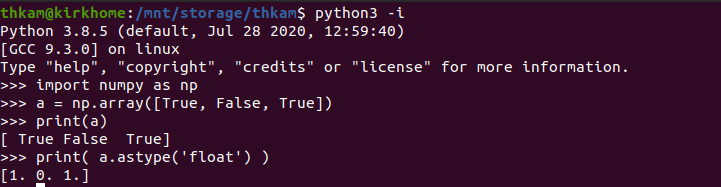
\includegraphics[width=0.7\linewidth]{astypefloat}
	\end{frame}


	\begin{frame}
	\frametitle{Μερικές επεξηγήσεις}
	\lstinputlisting[language=Python, firstline=11, lastline=20]{lecture2/fftexample.py}
	\begin{itemize}
		\item Στην συνέχεια ορίζουμε τον άξονα του χρόνου και τον άξονα των συχνοτήτων.
		\item ο άξονας του χρόνου αρχίζει από το -Τmax και φτάνει στο +Τmax.
		\item επομένως $\Delta t=2T_\mathrm{max}/N$ όπου $N$ το πλήθος των σημείων.  
		\item στη συνέχεια υπολογίζουμε το $\Delta f$ σύμφωνα με την σχέση $\Delta f\Delta t = 1/N$.
	\end{itemize}
	\end{frame}

	\begin{frame}
	\frametitle{Μερικές επεξηγήσεις}
	\lstinputlisting[language=Python, firstline=25, lastline=29]{lecture2/fftexample.py}
	\begin{itemize}
		\item Εδώ είναι το "ζουμί".
		\item κάνουμε αυτό που είπαμε με τον fft και τις μεταθέσεις των δειγμάτων ώστε να υπολογιστεί σωστά το φάσμα.
		\item Χ = Dt * np.fftshift(np.fft(np.fftshift(x)))
		\item Πολλαπλασιάζουμε με Dt επειδή στο ολοκλήρωμα του μετασχηματισμού Fourier υπάρχει και εκεί ένα $\mathrm{d}t$.
		\begin{equation}
		X(f) = \int_{-\infty}^{+\infty}x(t)\mathrm{e}^{-j2\pi ft}\mathrm{d}t
		\end{equation}	
		
	\end{itemize}
	\end{frame}

	\begin{frame}
	\frametitle{Annotations}
	\lstinputlisting[language=Python, firstline=31, lastline=42]{lecture2/fftexample.py}
	\begin{figure}
		\begin{subfigure}{0.49\linewidth}
			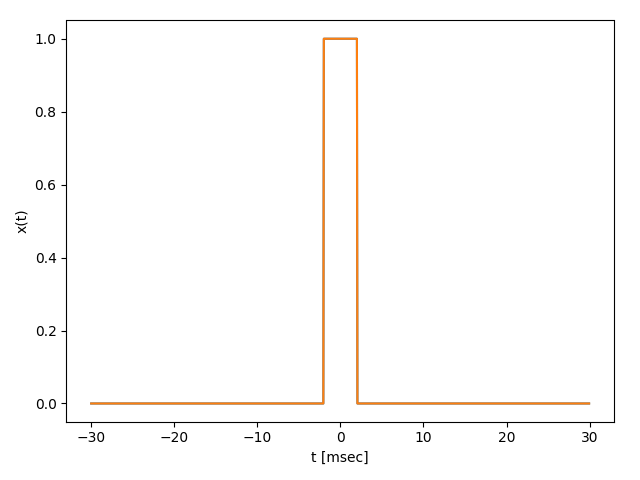
\includegraphics[width=\linewidth]{squarepulse}
		\end{subfigure}
		\begin{subfigure}{0.49\linewidth}
			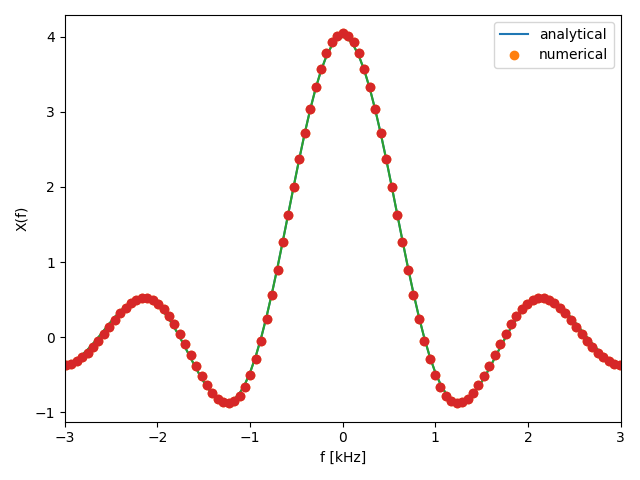
\includegraphics[width=\linewidth]{compsinc}
		\end{subfigure}
	\end{figure}
	\end{frame}

	\section{Python modules}
	
	\begin{frame}
		\frametitle{Το πρώτο μας Python module}
		\lstinputlisting[language=Python]{lecture2/commlib.py}
	\end{frame}

	\begin{frame}
	\frametitle{Διαβάζοντας το module}
	\lstinputlisting[language=Python]{lecture2/fftexamplemod.py}
	\end{frame}
	
	\section{Σήματα και Συστήματα}
	\begin{frame}
		\frametitle{Ένα παράδειγμα συστήματος}
		\begin{itemize}
			\item Ας δείξουμε τι συμβαίνει όταν ένα σήμα περνάει από ένα σύστημα.
			\item Θα θεωρήσουμε έναν τετραγωνικό παλμό στην είσοδο ενός συστήματος.
			\item Το σύστημα κόβει απότομα συχνότητες οι οποίες είναι μεγαλύτερες από μία τιμή $F_\mathrm{max}$.
			\item δηλαδή:
			\begin{equation}
			H(f)= \left\{
			\begin{array}{ll}
			1 & ,|f| \le F_\mathrm{max} \\
			0 & ,\text{διαφορετικά}\\
			\end{array} 
			\right. 
			\end{equation}
			\item Όταν για παράδειγμα ένα σήμα περνάει από ένα καλώδιο, "κόβονται" οι υψηλές συχνότητες. 
			\item Με διαφορετικό τρόπο βέβαια - όχι τόσο απότομα.
		\end{itemize}
	\end{frame}

	\begin{frame}
	\frametitle{Ένα παράδειγμα συστήματος}
	\begin{itemize}
		\item Αλλάζουμε λίγο την commlib προσθέτοντας:
		\begin{itemize} 
			\item μία πολύ απλή συνάρτηση για το τετραγωνικό μας φίλτρο (square\_filter).
			\item μία συνάρτηση για τον αντίστροφο μετασχηματισμό Fourier (inv\_spectrum).
			\item μία συνάρτηση που υλοποιεί την δράση του συστήματος πάνω σε ένα σήμα (system\_action).	
		\end{itemize}
	\end{itemize}
	\lstinputlisting[language=Python, firstline = 27, lastline = 43]{lecture2/commlib.py}
	
	\end{frame}

	\begin{frame}
	\frametitle{Ένα παράδειγμα συστήματος}
	\begin{itemize}
		\item Έτσι γράφουμε κώδικα που μπορούμε να επαναχρησιμοποιήσουμε.		
	\end{itemize}
	\lstinputlisting[language=Python]{lecture2/systemexample.py}
	\end{frame}

	\begin{frame}
		\frametitle{Python callables}
		\begin{itemize}
			\item Προσέξτε ότι περνάμε ως όρισμα μία συνάρτηση στην system\_action.
			\item μάλιστα αυτή η συνάρτηση ορίζεται μέσω ενός lambda.
			\item με το lambda ορίζουμε μία μικρή συνάρτηση που μπορεί να χρησιμοποιεί και παραμέτρους που έχουν οριστεί παραπάνω.
			\item Hc = lambda f : cl.square\_filter(f, Fmax) σημαίνει φτιάξε μία συνάρτηση με μία είσοδο την f η οποία να υπολογίζεται από την cl.square\_filter(f, Fmax)
			\item Με τον τρόπο αυτό περνάμε την κατάλληλη συνάρτηση μεταφοράς του φίλτρου στην system\_action.
		\end{itemize}
	\end{frame}

	\begin{frame}
		\frametitle{Αποτελέσματα}
		\begin{figure}
			\begin{subfigure}{0.49\linewidth}
				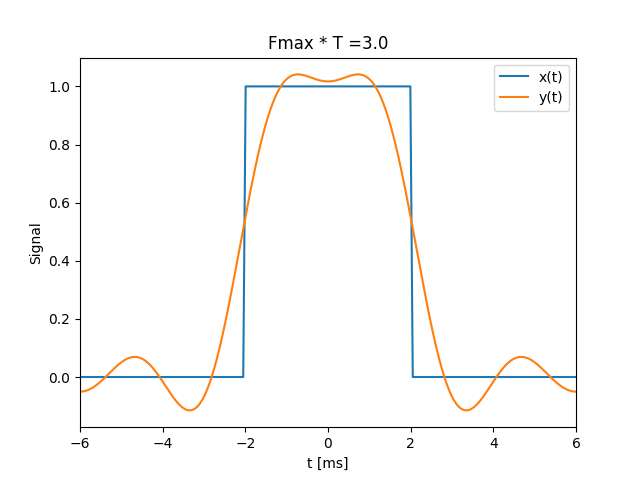
\includegraphics[width=\linewidth]{BT}
			\end{subfigure}
			\begin{subfigure}{0.49\linewidth}
				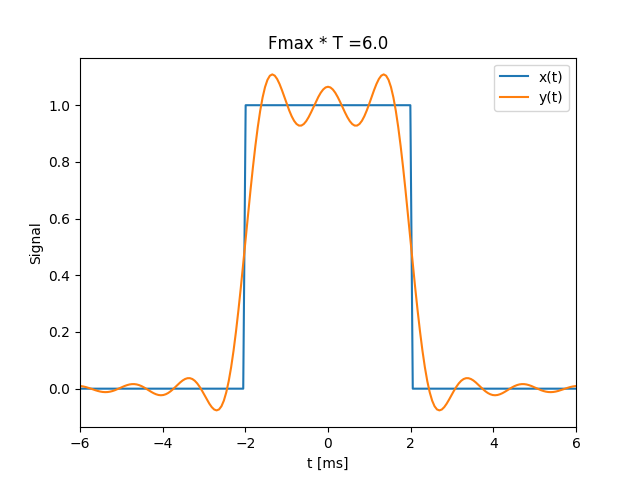
\includegraphics[width=\linewidth]{BT6}	
			\end{subfigure}		
		\end{figure}
	\end{frame}

	\begin{frame}
	\frametitle{Αποτελέσματα}
	\begin{figure}
		\begin{subfigure}{0.49\linewidth}
			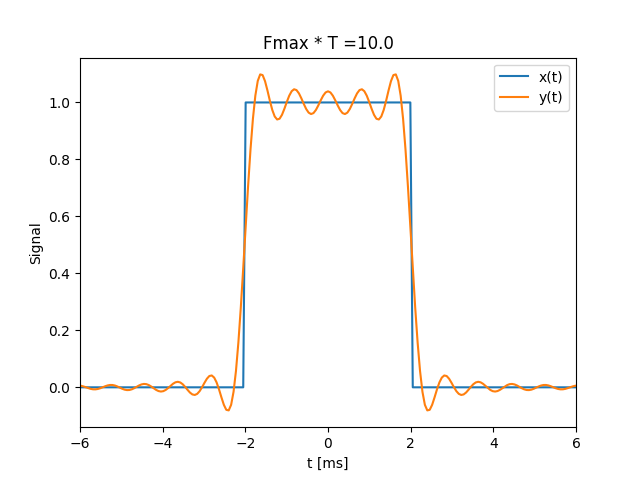
\includegraphics[width=\linewidth]{BT10}
		\end{subfigure}
		\begin{subfigure}{0.49\linewidth}
			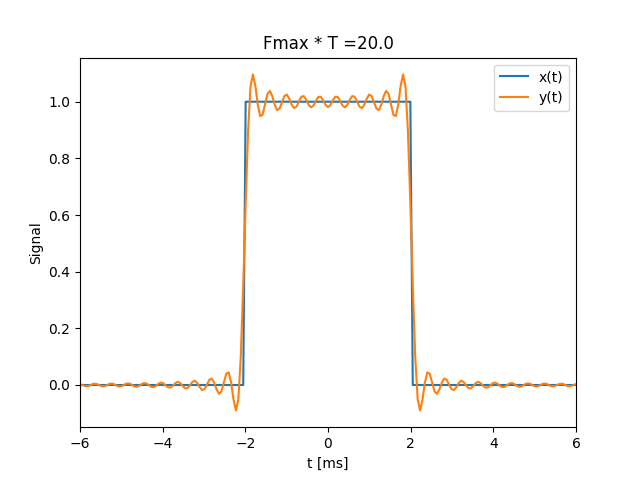
\includegraphics[width=\linewidth]{BT20}	
		\end{subfigure}		
	\end{figure}
	\end{frame}

	\begin{frame}
	\frametitle{Ερμηνεία με τα φάσματα}
	\lstinputlisting[language=Python]{lecture2/systemspecs.py}
	\end{frame}

	\begin{frame}
		\frametitle{Ερμηνεία με τα φάσματα}
		\begin{figure}
			\begin{subfigure}{0.49\linewidth}
				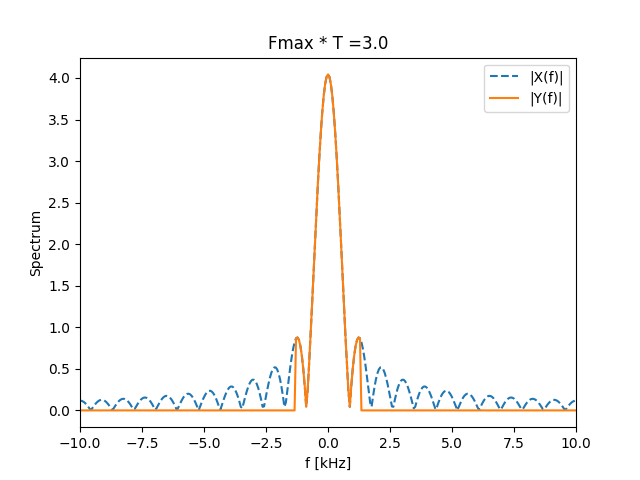
\includegraphics[width=\linewidth]{BT3s}
			\end{subfigure}
			\begin{subfigure}{0.49\linewidth}
				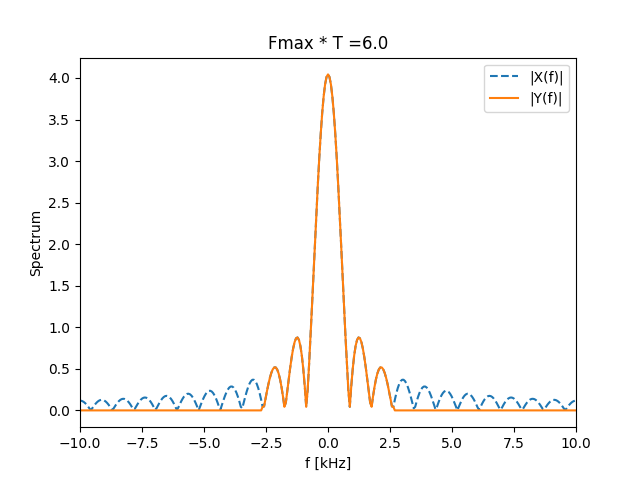
\includegraphics[width=\linewidth]{BT6s}	
			\end{subfigure}		
		\end{figure}
	\end{frame}

	\begin{frame}
	\frametitle{Ερμηνεία με τα φάσματα}
	\begin{figure}
		\begin{subfigure}{0.49\linewidth}
			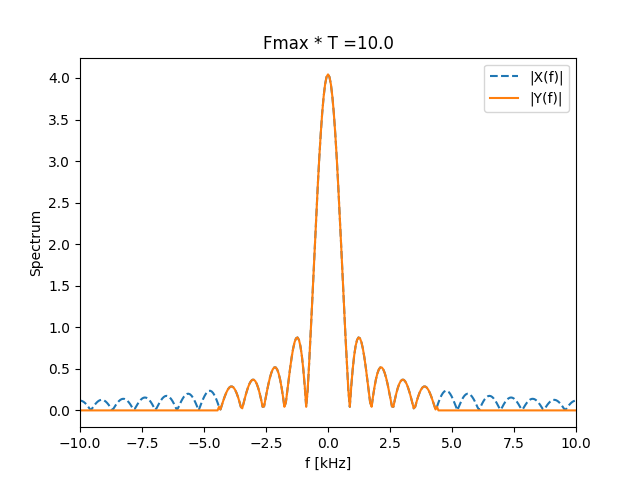
\includegraphics[width=\linewidth]{BT10s}
		\end{subfigure}
		\begin{subfigure}{0.49\linewidth}
			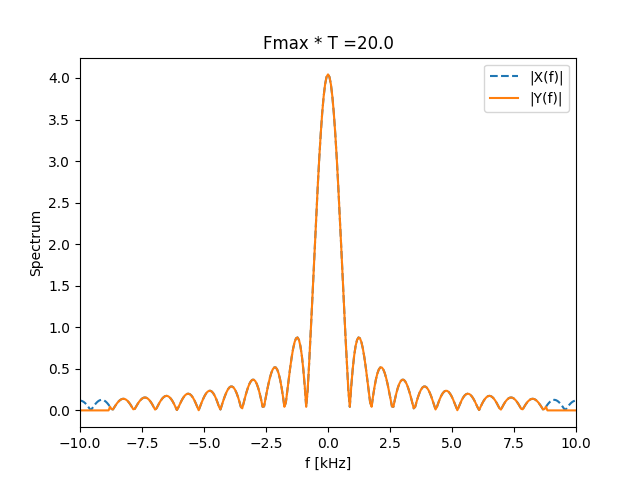
\includegraphics[width=\linewidth]{BT20s}	
		\end{subfigure}		
	\end{figure}
	\end{frame}
\end{document}

